\documentclass[11pt,a4paper,oneside]{report}

% ============================================================
% Material de estudio — Semana 4
% Unidad 2, Tema 1: Elicitación de requisitos
% Ingeniería de Requerimientos (ISR-401) · UTEQ · SPA 2026-2027
% Compilación: pdflatex -> bibtex -> pdflatex -> pdflatex
% ============================================================

\usepackage[utf8]{inputenc}
\usepackage[T1]{fontenc}
% babel no disponible en este entorno
\usepackage{mathptmx}
\usepackage[scaled]{helvet}
\usepackage{courier}
\renewcommand{\familydefault}{\sfdefault}
\usepackage[a4paper,top=2.8cm,bottom=2.6cm,inner=2.6cm,outer=2.2cm,headheight=28pt]{geometry}
\usepackage{graphicx}
\usepackage{array}
\usepackage{tabularx}
\usepackage{longtable}
\usepackage{colortbl}
\usepackage{xcolor}
\usepackage{enumitem}
\usepackage{fancyhdr}
\usepackage{lastpage}
\usepackage[most]{tcolorbox}
\usepackage{tikz}
\usetikzlibrary{positioning,shapes.geometric,arrows.meta,calc}
\usepackage[numbers,sort&compress]{natbib}
\usepackage{url}
\usepackage{needspace}
\usepackage{caption}
\usepackage{titlesec}
\usepackage[hidelinks]{hyperref}

% ---------- Textos en español (sin babel) ----------
\renewcommand{\tablename}{Tabla}
\renewcommand{\figurename}{Figura}
\renewcommand{\bibname}{Referencias}
\renewcommand{\contentsname}{Contenido}
\renewcommand{\chaptername}{Semana}

% ---------- Paleta institucional ----------
\definecolor{utegreen}{HTML}{0B7A3B}
\definecolor{utegreendk}{HTML}{075C2C}
\definecolor{midblue}{HTML}{1F5C8B}
\definecolor{gold}{HTML}{D4A017}
\definecolor{rowgray}{HTML}{EFEFEF}
\definecolor{boxgray}{HTML}{F4F6F4}
\definecolor{lightred}{HTML}{FBEAEA}
\definecolor{lightgold}{HTML}{FBF3DC}
\definecolor{lightblue}{HTML}{EAF1F7}
\definecolor{lightgreen}{HTML}{DCEFE3}

% ---------- Columnas ----------
\newcolumntype{L}[1]{>{\raggedright\arraybackslash}p{#1}}
\newcolumntype{C}[1]{>{\centering\arraybackslash}p{#1}}
\newcolumntype{Y}{>{\raggedright\arraybackslash}X}

% ---------- Títulos ----------
\titleformat{\chapter}[display]{\normalfont\bfseries\color{utegreendk}}{\Large SEMANA \thechapter}{4pt}{\huge}
\titlespacing*{\chapter}{0pt}{-10pt}{18pt}
\titleformat{\section}{\normalfont\Large\bfseries\color{utegreendk}}{\thesection}{0.6em}{}
\titleformat{\subsection}{\normalfont\large\bfseries\color{midblue}}{\thesubsection}{0.6em}{}
\setcounter{chapter}{3}

% ---------- Encabezado y pie ----------
\pagestyle{fancy}
\fancyhf{}
\lhead{\footnotesize UTEQ \,$\cdot$\, Ingeniería de Requerimientos (ISR-401)}
\rhead{\footnotesize Semana 4 \,$\cdot$\, Elicitación de requisitos}
\lfoot{\footnotesize Prof. Gleiston C. Guerrero-Ulloa, PhD}
\rfoot{\footnotesize Página \thepage\ de \pageref{LastPage}}
\renewcommand{\headrulewidth}{0.6pt}
\renewcommand{\footrulewidth}{0.4pt}
\fancypagestyle{plain}{\fancyhf{}\lfoot{\footnotesize Prof. Gleiston C. Guerrero-Ulloa, PhD}\rfoot{\footnotesize Página \thepage\ de \pageref{LastPage}}\renewcommand{\headrulewidth}{0pt}}

\setlength{\parindent}{0pt}
\setlength{\parskip}{5pt}
\setlength{\emergencystretch}{3em}
\renewcommand{\arraystretch}{1.25}

% ---------- Cajas ----------
\newcommand{\thdr}[1]{\cellcolor{utegreen}\textcolor{white}{\textbf{#1}}}
\newtcolorbox{definicion}[1][]{colback=lightgreen,colframe=utegreen,boxrule=0.8pt,arc=2mm,fonttitle=\bfseries,breakable,title={Definición},#1}
\newtcolorbox{enlapractica}[1][]{colback=lightblue,colframe=midblue,boxrule=0.8pt,arc=2mm,fonttitle=\bfseries,breakable,title={Cómo se hace en la práctica},#1}
\newtcolorbox{cuidado}[1][]{colback=lightgold,colframe=gold!80!black,boxrule=0.8pt,arc=2mm,fonttitle=\bfseries,breakable,title={Error frecuente},#1}
\newtcolorbox{cajapfc}[1][]{colback=boxgray,colframe=utegreendk,boxrule=0.8pt,arc=2mm,fonttitle=\bfseries,breakable,title={Aplicación al Proyecto Fin de Curso},#1}

\begin{document}

% ============================================================
% PORTADA
% ============================================================
\thispagestyle{empty}
\noindent
\includegraphics[width=\linewidth]{logoband.png}

\vspace{30pt}
\begin{center}
	{\large Facultad de Ciencias de la Computación \,$\cdot$\, Carrera de Software}\\[36pt]
	{\Huge\bfseries\textcolor{utegreendk}{Elicitación de requisitos}}\\[10pt]
	{\Large Fuentes y técnicas para descubrir lo que el sistema debe hacer}\\[30pt]
	{\large\bfseries Material de estudio de la semana 4}\\[4pt]
	{\large Unidad 2. Elicitación y Análisis de Requisitos \,$\cdot$\, Tema 1}\\[4pt]
	{\large 16 al 22 de noviembre de 2026}
\end{center}

\vspace{30pt}
\begin{center}
	\begin{tabular}{L{0.30\linewidth}L{0.55\linewidth}}
		\textbf{Asignatura} & Ingeniería de Requerimientos (ISR-401)\\
		\textbf{Nivel / paralelo} & Cuarto nivel / A\\
		\textbf{Periodo} & Segundo Periodo Académico Ordinario 2026--2027\\
		\textbf{Docente} & Gleiston Cicerón Guerrero Ulloa, PhD\\
	\end{tabular}
\end{center}

\vfill
\noindent\textcolor{gold}{\rule{\linewidth}{1.5pt}}
\begin{center}
	\small Resultado de aprendizaje de la unidad: aplica técnicas de elicitación y análisis de requisitos para identificar, clasificar y modelar requisitos.
\end{center}

\newpage
\tableofcontents
\newpage

% ============================================================
\chapter{Elicitación de requisitos}
% ============================================================

\section*{Antes de la clase}
\phantomsection\addcontentsline{toc}{section}{Antes de la clase}

Esta semana se trabaja con aula invertida: usted lee este material antes de la primera sesión y la clase se dedica a practicar. Lea las secciones 4.1 a 4.10 (unas dos horas de lectura) y responda el cuestionario corto del SGA antes de la primera sesión de la semana. Las secciones 4.11 a 4.13 se leen antes de iniciar el taller GA-TL-02.

\begin{tcolorbox}[colback=boxgray,colframe=utegreen,boxrule=0.8pt,arc=2mm,fonttitle=\bfseries,title={Al terminar la semana usted podrá}]
	\begin{enumerate}[leftmargin=18pt,itemsep=2pt]
		\item Identificar las fuentes de requisitos de un sistema real: partes interesadas, documentos, sistemas existentes, normas y leyes.
		\item Explicar en qué consiste cada técnica de elicitación del sílabo y cuándo conviene usarla.
		\item Diseñar un guion de entrevista estructurada con preguntas abiertas, neutrales y simples.
		\item Aplicar la fase de empatía del design thinking con un mapa de empatía y una pregunta «¿Cómo podríamos\ldots?».
		\item Seleccionar y combinar técnicas para el plan de elicitación del Proyecto Fin de Curso (PFC).
	\end{enumerate}
\end{tcolorbox}

% ------------------------------------------------------------
\section{Qué es elicitar y por qué es difícil}
% ------------------------------------------------------------

\begin{definicion}
	\textbf{Elicitar requisitos} es sacar a la luz, de forma ordenada, lo que las personas y los documentos saben sobre el problema y sobre lo que el sistema debe hacer. No es copiar lo que el cliente dicta: es un trabajo activo en el que el analista pregunta, observa, lee y prueba ideas con las partes interesadas \citep{pohl_2025,swebok_v4_2024}.
\end{definicion}

La norma ISO/IEC/IEEE 29148:2018 incluye la elicitación dentro del proceso de definición de necesidades y requisitos de las partes interesadas. En su apartado 6.3.3.3 indica que identificar las necesidades incluye obtenerlas directamente de las personas, pero también descubrir las necesidades implícitas a partir del conocimiento del dominio y del contexto \citep{iso29148_2018}. Esa segunda parte es la difícil: mucha información importante nadie la dice, porque se da por obvia.

Lo que una persona sabe pero no expresa se llama conocimiento tácito (o conocimiento implícito). Un cajero de una cooperativa sabe que los lunes por la mañana la fila se triplica y que entonces se salta un paso de verificación; nunca lo mencionará en una entrevista si no se le pregunta por los lunes. La guía SWEBOK lo resume así: los usuarios pueden tener dificultad para describir sus tareas, omitir información importante o no estar dispuestos a colaborar, y muchos requisitos son tácitos \citep{swebok_v4_2024}. Ferrari, Spoletini y Gnesi mostraron, además, que las ambigüedades que el analista detecta durante una entrevista no son solo un problema: si se atienden con nuevas preguntas, sirven para descubrir conocimiento tácito \citep{ferrari_2016}.

\begin{enlapractica}
	Cuando una respuesta le parezca obvia o vaga («lo normal», «como siempre», «rápido»), no la anote y siga: pida un ejemplo concreto («¿me cuenta la última vez que pasó?») o una cifra («¿cuánto es rápido para usted?»). Ahí suele estar el conocimiento tácito.
\end{enlapractica}

Por todo esto, ninguna técnica basta sola. Las revisiones de la literatura sobre elicitación (estudios que reúnen y comparan lo publicado sobre un tema) muestran que la eficacia de cada técnica depende de la situación, por lo que en la práctica se eligen según el contexto y se combinan \citep{zowghi_coulin_2005,pacheco_2018}.

% ------------------------------------------------------------
\section{Fuentes de requisitos}
% ------------------------------------------------------------

Una fuente de requisitos es cualquier persona, documento o sistema del que se puede obtener información sobre lo que el sistema debe hacer o sobre las condiciones que debe cumplir \citep{ireb_cpre_fl_2026,pohl_2025}. El sílabo agrupa las fuentes en cuatro tipos, que la Tabla~\ref{tab:fuentes} resume con ejemplos de nuestra región.

{\small
	\begin{longtable}{|L{0.18\linewidth}|L{0.38\linewidth}|L{0.34\linewidth}|}
		\caption{Tipos de fuentes de requisitos, con ejemplos del entorno de Quevedo y Los Ríos.}\label{tab:fuentes}\\
		\hline
		\thdr{Fuente} & \thdr{Qué aporta} & \thdr{Ejemplos}\\
		\hline
		\endfirsthead
		\hline
		\thdr{Fuente} & \thdr{Qué aporta} & \thdr{Ejemplos}\\
		\hline
		\endhead
		Partes interesadas (stakeholders) & Necesidades, objetivos, problemas actuales, prioridades y criterios de aceptación. Son la fuente principal, pero también la más sesgada si se consulta a una sola. & Gerente de una cooperativa de cacao, técnico de acopio, socio productor, contador, auditor de la certificación.\\
		\hline
		\rowcolor{rowgray} Documentos & Reglas de negocio, datos que se manejan, formatos, flujos formales del proceso. & Reglamento interno, formularios en papel, actas de asamblea, manual de procesos, reportes mensuales.\\
		\hline
		Sistemas existentes & Funciones que ya se usan, datos y sus estructuras, problemas conocidos, interfaces con otros sistemas. & Hoja de cálculo de liquidaciones, sistema contable, registro de errores, portal del SRI con el que hay que integrarse.\\
		\hline
		\rowcolor{rowgray} Normas, leyes y estándares & Restricciones obligatorias y requisitos de calidad que no son negociables. & Ley Orgánica de Protección de Datos Personales \citep{lopdp_2021}, normativa tributaria, ISO/IEC 25010, normas de una certificación de comercio justo.\\
		\hline
	\end{longtable}
}

\subsection{Partes interesadas: quiénes son y cuántas consultar}

Una parte interesada es una persona u organización que influye en el sistema o que se ve afectada por él. La norma 29148 pide identificar a las partes interesadas de todo el ciclo de vida del sistema (no solo a quienes lo usarán), y advierte que la información obtenida de una sola clase de partes interesadas, o de un solo nivel de la organización, tiende a estar sesgada; por eso recomienda consultar a una muestra representativa de cada clase y de varios niveles (apartado 6.3.3.2) \citep{iso29148_2018}.

\begin{enlapractica}
	Haga una lista de roles, no de nombres: quién decide (gerente), quién usa el sistema todos los días (técnico, cajero), quién recibe sus resultados (socio, cliente), quién lo mantiene (soporte de TI) y quién lo controla desde fuera (auditor, ente regulador). Para cada rol anote su interés, su influencia y su disponibilidad. Esa lista es la base de la matriz poder--interés que se pide en la entrega TA-PFC-E1.
\end{enlapractica}

\subsection{Documentos, sistemas existentes y normas}

Las fuentes que no son personas se consultan con técnicas basadas en artefactos, que se ven en la sección~\ref{sec:artefactos}. La guía SWEBOK incluye entre ellas las versiones anteriores del sistema, los registros de defectos, los sistemas con los que el nuevo debe comunicarse, la comparación con productos de la competencia, la búsqueda bibliográfica y las normas y regulaciones aplicables \citep{swebok_v4_2024}. La norma 29148 añade que muchas restricciones importantes las imponen otros sistemas del entorno y no las personas (apartado 6.3.3.5) \citep{iso29148_2018}.

\begin{cuidado}
	Pensar que «el cliente» es una sola persona. Si solo entrevista al gerente, obtendrá los requisitos que el gerente imagina, no los que necesita quien hace el trabajo. Las contradicciones entre partes interesadas no son un fracaso de la elicitación: son información valiosa que se resuelve en la semana 5, con el análisis y la negociación.
\end{cuidado}

% ------------------------------------------------------------
\section{Mapa de las técnicas de elicitación}
% ------------------------------------------------------------

El temario de certificación del International Requirements Engineering Board (IREB), en su sección 4.2, clasifica las técnicas en dos grandes grupos: las técnicas de recolección, que obtienen información que ya existe en las personas o en los documentos, y las técnicas de diseño y generación de ideas, que crean propuestas nuevas para descubrir lo que todavía nadie ha pensado \citep{ireb_cpre_fl_2026}. La Figura~\ref{fig:mapa} ubica en ese esquema las técnicas que pide el sílabo.

\begin{figure}[h]
	\centering
	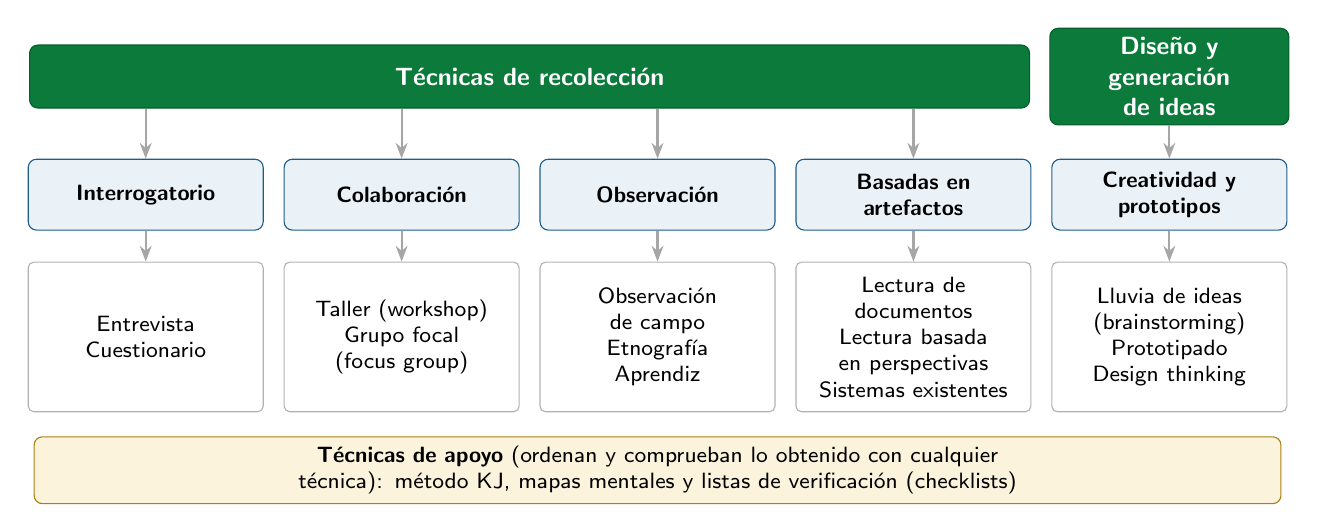
\begin{tikzpicture}[
		grupo/.style={draw=utegreendk,fill=utegreen,text=white,rounded corners=3pt,minimum height=0.8cm,align=center,font=\small\bfseries},
		cat/.style={draw=midblue,fill=lightblue,rounded corners=3pt,text width=2.75cm,align=center,minimum height=0.9cm,font=\footnotesize\bfseries},
		tec/.style={draw=gray!60,fill=white,rounded corners=2pt,text width=2.75cm,align=center,font=\footnotesize,minimum height=1.9cm,anchor=north},
		flecha/.style={-{Stealth[length=2mm]},draw=gray!70,thick}
		]
		\foreach \i/\x in {1/1.5,2/4.75,3/8.0,4/11.25,5/14.5} {\coordinate (x\i) at (\x,0);}
		\node[grupo,minimum width=12.7cm] (rec) at (6.375,0) {Técnicas de recolección};
		\node[grupo,minimum width=3.0cm,text width=2.8cm] (dis) at (14.5,0) {Diseño y\\generación de ideas};
		\node[cat] (c1) at (1.5,-1.5) {Interrogatorio};
		\node[cat] (c2) at (4.75,-1.5) {Colaboración};
		\node[cat] (c3) at (8.0,-1.5) {Observación};
		\node[cat] (c4) at (11.25,-1.5) {Basadas en artefactos};
		\node[cat] (c5) at (14.5,-1.5) {Creatividad y prototipos};
		\node[tec] (t1) at (1.5,-2.35) {Entrevista\\Cuestionario};
		\node[tec] (t2) at (4.75,-2.35) {Taller (workshop)\\Grupo focal\\(focus group)};
		\node[tec] (t3) at (8.0,-2.35) {Observación de campo\\Etnografía\\Aprendiz};
		\node[tec] (t4) at (11.25,-2.35) {Lectura de documentos\\Lectura basada en perspectivas\\Sistemas existentes};
		\node[tec] (t5) at (14.5,-2.35) {Lluvia de ideas (brainstorming)\\Prototipado\\Design thinking};
		\node[draw=gold!80!black,fill=lightgold,rounded corners=3pt,text width=15.6cm,align=center,font=\footnotesize,minimum height=0.8cm] (apoyo) at (8.0,-5.0) {\textbf{Técnicas de apoyo} (ordenan y comprueban lo obtenido con cualquier técnica): método KJ, mapas mentales y listas de verificación (checklists)};
		\foreach \c in {c1,c2,c3,c4} {\draw[flecha] (rec.south -| \c) -- (\c.north);}
		\draw[flecha] (dis) -- (c5);
		\foreach \c/\t in {c1/t1,c2/t2,c3/t3,c4/t4,c5/t5} {\draw[flecha] (\c) -- (\t);}
	\end{tikzpicture}
	\caption{Técnicas del sílabo ubicadas en la clasificación del temario IREB \citep{ireb_cpre_fl_2026}. Las técnicas de apoyo se agrupan aparte, como en el sílabo.}\label{fig:mapa}
\end{figure}

La norma 29148, por su parte, recomienda considerar varias técnicas porque las fuentes son diversas, y menciona como ejemplos los talleres estructurados con lluvia de ideas, las entrevistas, los cuestionarios, la observación del entorno de trabajo, la revisión de documentación técnica, el análisis de mercado, la simulación, el prototipado y el modelado (apartado 6.3.3.5) \citep{iso29148_2018}.

% ------------------------------------------------------------
\needspace{10\baselineskip}
\section{Técnicas de interrogatorio: entrevista y cuestionario}
% ------------------------------------------------------------

\subsection{La entrevista}

\begin{definicion}
	Una \textbf{entrevista} es una conversación planificada entre el analista y una parte interesada para obtener información sobre el problema, el trabajo actual y lo que se espera del sistema \citep{wiegers_beatty_2013,zowghi_coulin_2005}.
\end{definicion}

Según cuánto se fija de antemano, la entrevista puede ser estructurada (preguntas fijas en un orden fijo, iguales para todos los entrevistados), semiestructurada (un guion de temas que permite repreguntar) o no estructurada (conversación abierta sobre el problema). La estructurada permite comparar las respuestas de varias personas del mismo rol; la semiestructurada es la más usada porque combina orden y flexibilidad \citep{zowghi_coulin_2005,wiegers_beatty_2013}. En el taller GA-TL-02 usted diseñará una entrevista estructurada, con espacio controlado para las repreguntas.

\begin{enlapractica}
	Un guion de entrevista tiene tres partes:
	\begin{enumerate}[leftmargin=18pt,itemsep=2pt]
		\item \textbf{Apertura} (unos 5 minutos): presentación, propósito, tiempo estimado, lectura del consentimiento informado y permiso para grabar.
		\item \textbf{Bloques temáticos} (unos 30 minutos): de lo general a lo particular (secuencia en embudo). Por ejemplo: el trabajo actual, los problemas, las excepciones, los datos que se manejan y las expectativas sobre el sistema.
		\item \textbf{Cierre} (unos 5 minutos): resumen de lo entendido para que el entrevistado lo confirme, pregunta final («¿qué no le pregunté y debí preguntarle?»), a quién más conviene entrevistar y agradecimiento.
	\end{enumerate}
\end{enlapractica}

\paragraph{Tipos de preguntas.} Las preguntas abiertas («¿cómo registra hoy una entrega de cacao?») hacen hablar al entrevistado y revelan el proceso real; las cerradas («¿lo registra en papel o en el computador?») confirman un dato concreto; las de sondeo o repregunta («¿por qué?», «¿qué pasa si\ldots?», «¿me da un ejemplo?») profundizan. Un buen guion empieza con abiertas, usa cerradas para confirmar y deja espacio para el sondeo.

\paragraph{Errores frecuentes.} Bano y colaboradores observaron entrevistas de elicitación hechas por estudiantes en juego de roles durante dos semestres e identificaron 34 errores distintos, agrupados en siete temas; los estudiantes tuvieron más dificultades con la formulación de las preguntas, con las preguntas que omitieron y con el orden de la entrevista, y no mejoraron de forma espontánea de una entrevista a la siguiente \citep{bano_2019}. Por eso el taller de esta semana incluye un paso explícito de corrección de preguntas. La Tabla~\ref{tab:preguntas} muestra ejemplos de preguntas mal formuladas y cómo corregirlas.

{\small
	\begin{longtable}{|L{0.30\linewidth}|L{0.22\linewidth}|L{0.38\linewidth}|}
		\caption{Preguntas defectuosas y su corrección (caso: centro de acopio de cacao).}\label{tab:preguntas}\\
		\hline
		\thdr{Pregunta defectuosa} & \thdr{Defecto} & \thdr{Versión corregida}\\
		\hline
		\endfirsthead
		\hline
		\thdr{Pregunta defectuosa} & \thdr{Defecto} & \thdr{Versión corregida}\\
		\hline
		\endhead
		¿Verdad que sería mejor registrar las entregas en una aplicación móvil? & Inductiva: sugiere la respuesta y además propone la solución. & ¿Cómo registra hoy una entrega de cacao, desde que llega el socio hasta que se le paga?\\
		\hline
		\rowcolor{rowgray} ¿Cuánto tarda el pesaje y quién revisa la humedad? & Doble: dos preguntas en una; el entrevistado responderá solo una. & ¿Cuánto tarda el pesaje? (y después, por separado) ¿Quién revisa la humedad y cómo lo hace?\\
		\hline
		¿El sistema actual es lento? & Cerrada sin necesidad y vaga («lento»). & ¿En qué momentos del día el registro le toma más tiempo? ¿Cuánto tiempo, aproximadamente?\\
		\hline
		\rowcolor{rowgray} ¿Necesita un módulo de reportes con dashboard y exportación a Excel? & Técnica: usa términos del analista y habla de la solución. & ¿Qué información le pide la gerencia cada mes y cómo la prepara hoy?\\
		\hline
		¿No tiene ningún problema con los socios? & Negativa y cerrada; induce a responder «no». & Cuénteme la última vez que hubo un desacuerdo con un socio sobre el peso o el precio. ¿Qué pasó?\\
		\hline
	\end{longtable}
}

\paragraph{Registro.} Durante la entrevista una persona pregunta y otra registra. Con el consentimiento del entrevistado se graba el audio, y después se redacta una minuta o transcripción con citas textuales de lo importante. Las grabaciones y los consentimientos firmados no se suben al repositorio público: se guardan en la carpeta institucional privada y en el repositorio se registra un manifiesto (sección~\ref{sec:etica}).

\subsection{El cuestionario}

\begin{definicion}
	Un \textbf{cuestionario} es un conjunto de preguntas escritas que muchas personas responden por su cuenta, en papel o en línea \citep{zowghi_coulin_2005,ireb_cpre_fl_2026}.
\end{definicion}

El cuestionario sirve para llegar a muchas personas dispersas (por ejemplo, 200 socios de una cooperativa que viven en recintos distintos) y para medir cuántas comparten un problema o una preferencia que ya se identificó con entrevistas. No sirve para descubrir lo desconocido: nadie responde a lo que no se le pregunta. Por eso se usa después de las entrevistas, no en su lugar.

\begin{enlapractica}
	Diseñe preguntas cortas y de una sola idea; use escalas (por ejemplo, de 1 «nunca» a 5 «siempre») para lo que quiere medir y deje una o dos preguntas abiertas al final. Antes de enviarlo, pruébelo con dos o tres personas del mismo perfil (prueba piloto) para detectar preguntas que se entienden mal. Herramientas como los formularios de Microsoft o de Google sirven; la tabulación se guarda en el repositorio sin datos personales.
\end{enlapractica}

\begin{cuidado}
	Reemplazar la entrevista por un formulario en línea. Un cuestionario respondido por personas que el analista nunca escuchó produce cifras sin contexto; en la práctica experimental de la unidad 2 y en el PFC se exige, además, la aplicación real de la entrevista.
\end{cuidado}

% ------------------------------------------------------------
\section{Técnicas de colaboración: taller y grupo focal}
% ------------------------------------------------------------

\subsection{Taller de requisitos}

Un taller de requisitos (workshop) es una reunión planificada y conducida por un facilitador en la que varias partes interesadas trabajan juntas para obtener, discutir y acordar requisitos en poco tiempo \citep{wiegers_beatty_2013,zowghi_coulin_2005}. Su ventaja es que los desacuerdos salen a la luz y se discuten en la misma sesión; su riesgo es que las personas con más poder dominen la conversación.

\begin{enlapractica}
	Defina un objetivo concreto para el taller («acordar los pasos del registro de una entrega y sus excepciones»), una agenda con tiempos, los roles (facilitador neutral, quien registra, quien controla el tiempo) y las reglas (todos hablan, se critica la idea y no a la persona). Cierre con una lista de acuerdos y de temas pendientes, con responsable y fecha.
\end{enlapractica}

\subsection{Grupo focal}

Un grupo focal (focus group) reúne a unas seis a diez personas de un mismo perfil para conversar, guiadas por un moderador, sobre sus experiencias, necesidades y reacciones ante una idea. A diferencia del taller, su propósito no es acordar requisitos sino conocer opiniones y percepciones de un tipo de usuario \citep{zowghi_coulin_2005}. La guía SWEBOK lo incluye entre las técnicas comunes de elicitación (sección 2.2) \citep{swebok_v4_2024}.

\begin{enlapractica}
	Use el grupo focal con usuarios finales que no tienen poder de decisión y a los que es difícil entrevistar uno por uno (por ejemplo, socios productores en un día de acopio). Prepare de 5 a 8 preguntas abiertas, muestre si puede un prototipo en papel para provocar reacciones y registre en audio con consentimiento de todos.
\end{enlapractica}

% ------------------------------------------------------------
\section{Técnicas de observación: observación y etnografía}
% ------------------------------------------------------------

La observación consiste en mirar a las personas mientras hacen su trabajo real, en su lugar de trabajo, para descubrir lo que no dirían en una entrevista: pasos que se saltan, atajos, papeles pegados al monitor, interrupciones \citep{zowghi_coulin_2005,robertson_2025}. Puede ser pasiva (el analista solo mira y anota) o participativa; en la variante llamada aprendiz (apprenticing), el analista aprende a hacer el trabajo bajo la guía de quien lo realiza y le pregunta mientras lo hace \citep{robertson_2025}.

La etnografía es una forma más larga y profunda de observación, tomada de la antropología: el analista convive con el grupo durante un periodo para entender su cultura de trabajo, sus reglas no escritas y la manera en que realmente colaboran \citep{zowghi_coulin_2005}. En un proyecto de un semestre no se puede hacer una etnografía completa, pero sí una observación de campo de varias horas con enfoque etnográfico: describir lo que se ve sin juzgarlo y preguntar por qué se hace así.

\begin{enlapractica}
	Pida permiso, explique que observará el trabajo y no evaluará a las personas, y lleve una guía de observación con lo que va a registrar: actividad, quién la hace, con qué herramienta o documento, cuánto tarda, qué la interrumpe y qué improvisan. Tome fotografías solo de objetos y documentos, nunca de rostros sin consentimiento.
\end{enlapractica}

% ------------------------------------------------------------
\section{Técnicas basadas en artefactos y lectura basada en perspectivas}\label{sec:artefactos}
% ------------------------------------------------------------

Las técnicas basadas en artefactos obtienen requisitos de cosas que ya existen: documentos, formularios, reportes, sistemas en uso, registros de errores o productos de la competencia \citep{ireb_cpre_fl_2026,swebok_v4_2024}. Leer el reglamento de una cooperativa, por ejemplo, permite encontrar reglas de negocio (cómo se calcula una liquidación) sin ocupar el tiempo del gerente.

\subsection{Lectura basada en perspectivas}

\begin{definicion}
	La \textbf{lectura basada en perspectivas} (perspective-based reading) es una forma de leer un documento asumiendo, por turnos, el punto de vista de distintas personas que lo usarán (por ejemplo, el usuario, el diseñador y quien prueba el sistema), cada una con preguntas propias. Fue propuesta y evaluada experimentalmente por Basili y colaboradores para revisar documentos de requisitos \citep{basili_1996}.
\end{definicion}

En elicitación se usa para leer los documentos de la organización de forma sistemática y no superficial. Cada integrante del equipo lee el mismo documento con una perspectiva distinta y una lista de preguntas, y después se comparan los hallazgos.

{\small
	\begin{longtable}{|L{0.20\linewidth}|L{0.70\linewidth}|}
		\caption{Ejemplo de perspectivas para leer el reglamento de acopio de una cooperativa.}\label{tab:pbr}\\
		\hline
		\thdr{Perspectiva} & \thdr{Preguntas que guían la lectura}\\
		\hline
		\endfirsthead
		\hline
		\thdr{Perspectiva} & \thdr{Preguntas que guían la lectura}\\
		\hline
		\endhead
		Usuario (técnico de acopio) & ¿Qué pasos debo seguir? ¿Qué datos registro? ¿Qué hago si algo sale mal (cacao húmedo, socio sin carné)?\\
		\hline
		\rowcolor{rowgray} Diseñador del sistema & ¿Qué datos aparecen y qué relación tienen? ¿Qué reglas de cálculo hay? ¿Qué decisiones dependen de quién?\\
		\hline
		Probador (tester) & ¿Cómo comprobaría que el sistema aplica bien cada regla? ¿Qué cifras o umbrales concretos da el reglamento? ¿Qué casos límite hay?\\
		\hline
	\end{longtable}
}

% ------------------------------------------------------------
\section{Design thinking}
% ------------------------------------------------------------

\begin{definicion}
	El \textbf{design thinking} (pensamiento de diseño) es un enfoque centrado en las personas que avanza en cinco fases: empatizar, definir, idear, prototipar y probar. La guía SWEBOK lo incluye entre las técnicas de elicitación \citep{swebok_v4_2024}, y el temario IREB lo menciona como un concepto más amplio dentro de las técnicas de diseño y generación de ideas \citep{ireb_cpre_fl_2026}.
\end{definicion}

Hehn y colaboradores sostienen que el design thinking y la ingeniería de requisitos se complementan y proponen tres maneras de integrarlos \citep{hehn_2020}. Parizi y colaboradores revisaron 127 estudios publicados entre 2010 y 2021 en un mapeo sistemático (una revisión que clasifica todo lo publicado sobre un tema) y encontraron que la forma más frecuente de usarlo es al inicio, antes de definir los requisitos técnicos, para entender a los usuarios, generar ideas y probarlas con prototipos; para comprender el problema se usan sobre todo la lluvia de ideas, los mapas de empatía, las entrevistas y las personas (perfiles ficticios que representan a un tipo de usuario) \citep{parizi_2022}. El mismo estudio advierte sus dificultades: llegar a los usuarios finales adecuados, la presión de tiempo y que produce poca documentación formal, lo que complica la trazabilidad de los requisitos \citep{parizi_2022}. En una encuesta a profesionales brasileños, estos reportaron que el design thinking les ayudó a mejorar la obtención y la especificación de requisitos \citep{pereira_2021}.

{\small
	\begin{longtable}{|L{0.13\linewidth}|L{0.37\linewidth}|L{0.40\linewidth}|}
		\caption{Fases del design thinking y su producto en la elicitación.}\label{tab:dt}\\
		\hline
		\thdr{Fase} & \thdr{Qué se hace} & \thdr{Producto útil para los requisitos}\\
		\hline
		\endfirsthead
		\hline
		\thdr{Fase} & \thdr{Qué se hace} & \thdr{Producto útil para los requisitos}\\
		\hline
		\endhead
		Empatizar & Escuchar y observar a los usuarios en su contexto real. & Mapa de empatía: qué dice, qué piensa, qué hace y qué siente el usuario; sus dolores y lo que espera ganar.\\
		\hline
		\rowcolor{rowgray} Definir & Sintetizar lo aprendido en un problema centrado en el usuario. & Declaración del problema y pregunta «¿Cómo podríamos\ldots?» (How might we).\\
		\hline
		Idear & Generar muchas ideas de solución sin juzgarlas. & Lista de ideas agrupadas y elegidas por el equipo y el usuario.\\
		\hline
		\rowcolor{rowgray} Prototipar & Construir algo barato que se pueda mostrar. & Prototipo en papel o maqueta de pantallas.\\
		\hline
		Probar & Mostrar el prototipo al usuario y escuchar su reacción. & Retroalimentación: requisitos confirmados, corregidos y necesidades nuevas.\\
		\hline
	\end{longtable}
}

\begin{enlapractica}
	Para el mapa de empatía, divida una hoja en cuatro cuadrantes (dice, piensa, hace, siente) y añada abajo dos franjas (dolores y ganancias). Llénelo solo con lo que escuchó u observó, citando frases textuales cuando pueda. Después escriba la pregunta de diseño, por ejemplo: «¿Cómo podríamos lograr que el técnico de acopio registre una entrega sin hacer esperar al socio más de cinco minutos?». La pregunta habla de la persona y de su necesidad, no de la tecnología.
\end{enlapractica}

\begin{cuidado}
	Escribir la definición del problema como una solución: «¿Cómo podríamos hacer una app móvil para el acopio?». Esa pregunta ya decidió la tecnología y cierra la puerta a otras soluciones. Tampoco vale un mapa de empatía llenado por el equipo con lo que «cree» que siente el usuario: debe salir de lo dicho u observado.
\end{cuidado}

% ------------------------------------------------------------
\section{Técnicas de apoyo}
% ------------------------------------------------------------

Las técnicas de apoyo no obtienen información por sí solas: ayudan a generar ideas, a ordenar lo obtenido o a comprobar que no falta nada.

\paragraph{Lluvia de ideas (brainstorming).} Un grupo produce, en poco tiempo y sin criticar, la mayor cantidad posible de ideas sobre una pregunta; la evaluación se hace después. La norma 29148 la menciona dentro de los talleres estructurados \citep{iso29148_2018} y la guía SWEBOK, dentro de las reuniones de elicitación \citep{swebok_v4_2024}.

\paragraph{Prototipado.} Un prototipo es una versión parcial y barata del sistema (desde dibujos en papel hasta pantallas navegables) que se muestra a las partes interesadas para que reaccionen ante algo concreto. En elicitación se usa el prototipo exploratorio, que se descarta después de aprender de él \citep{swebok_v4_2024,wiegers_beatty_2013}.

\paragraph{Método KJ (diagrama de afinidad).} Propuesto por el antropólogo japonés Jiro Kawakita, consiste en escribir cada dato o idea en una tarjeta, agrupar las tarjetas por afinidad sin categorías previas, nombrar cada grupo y relacionar los grupos entre sí \citep{scupin_1997}. En elicitación sirve para ordenar decenas de hallazgos de entrevistas y observaciones y descubrir temas comunes.

\paragraph{Mapas mentales.} Diagrama que parte de un tema central y se ramifica en subtemas. Es útil para preparar los bloques temáticos de un guion de entrevista o para tomar notas durante un taller.

\paragraph{Listas de verificación (checklists).} Lista de preguntas o temas que no deben olvidarse. Por ejemplo, revisar al cerrar la elicitación si se preguntó por cada característica de calidad de ISO/IEC 25010 (desempeño, seguridad, usabilidad\ldots), que la norma 29148 recomienda usar para descubrir requisitos de calidad que suelen quedar implícitos (apartado 6.3.3.3) \citep{iso29148_2018}.

\begin{enlapractica}
	Después de las entrevistas, copie cada hallazgo en una nota adhesiva (física o en una pizarra digital como Miro o Excalidraw), agrúpelas con el método KJ y revise el resultado con una lista de verificación de las características de calidad. Cada grupo resultante es un candidato a área funcional del sistema; cada nota sin grupo merece una pregunta adicional.
\end{enlapractica}

% ------------------------------------------------------------
\section{Cómo seleccionar y combinar técnicas}
% ------------------------------------------------------------

No existe una técnica mejor que las demás. La revisión de Pacheco, García y Reyes, que analizó 140 estudios publicados entre 1993 y 2015, concluye que la eficacia de cada técnica depende de la situación: del producto que se desarrolla, de las características de las partes interesadas y del tipo de información que se busca \citep{pacheco_2018}. La Tabla~\ref{tab:seleccion} resume criterios prácticos para el plan de elicitación del PFC.

{\small
	\begin{longtable}{|L{0.20\linewidth}|L{0.33\linewidth}|L{0.37\linewidth}|}
		\caption{Guía práctica para elegir técnicas en el PFC.}\label{tab:seleccion}\\
		\hline
		\thdr{Técnica} & \thdr{Úsela cuando\ldots} & \thdr{Evítela o compleméntela cuando\ldots}\\
		\hline
		\endfirsthead
		\hline
		\thdr{Técnica} & \thdr{Úsela cuando\ldots} & \thdr{Evítela o compleméntela cuando\ldots}\\
		\hline
		\endhead
		Entrevista & Necesita entender el problema, el proceso y las prioridades de un rol clave. & El conocimiento es tácito o rutinario: complemente con observación.\\
		\hline
		\rowcolor{rowgray} Cuestionario & Necesita saber cuántas personas comparten algo ya identificado. & Aún no sabe qué preguntar: entreviste primero.\\
		\hline
		Taller & Varios roles deben acordar un proceso o resolver desacuerdos. & Hay mucha diferencia de poder entre participantes: entreviste por separado antes.\\
		\hline
		\rowcolor{rowgray} Grupo focal & Quiere conocer percepciones de un tipo de usuario numeroso. & Necesita decisiones: el grupo focal no decide.\\
		\hline
		Observación y etnografía & El trabajo es manual, rutinario o las personas no saben explicarlo. & No hay permiso para estar en el lugar de trabajo.\\
		\hline
		\rowcolor{rowgray} Lectura basada en perspectivas & Hay reglamentos, manuales o formularios que contienen reglas de negocio. & Los documentos están desactualizados: confírmelos con entrevistas.\\
		\hline
		Design thinking & El problema no está claro y hay que descubrir necesidades no expresadas. & El cliente solo puede dar una reunión corta: use una versión reducida (empatía y prueba).\\
		\hline
		\rowcolor{rowgray} Prototipado & Las personas no imaginan el sistema hasta verlo. & El cliente confunde el prototipo con el producto terminado: aclárelo siempre.\\
		\hline
	\end{longtable}
}

Una secuencia habitual en un proyecto como el PFC es: leer los documentos de la organización, entrevistar a los roles clave, observar el trabajo real, aplicar una sesión breve de design thinking con usuarios finales y, por último, confirmar con un cuestionario o con un taller lo que se encontró. La entrega TA-PFC-E1 le pide justificar qué técnica aplicará a cada parte interesada y por qué.

% ------------------------------------------------------------
\section{Inteligencia artificial en la elicitación: apoyo, no sustituto}
% ------------------------------------------------------------

La investigación reciente explora cómo los modelos de lenguaje de gran tamaño (large language models, LLM) pueden apoyar la elicitación: preparar guiones, transcribir y resumir entrevistas o extraer requisitos candidatos de un texto \citep{siddeshwar_2024,cheng_genai_re_2026}. Korn, Gorsch y Vogelsang construyeron un asistente que conduce entrevistas de elicitación y lo probaron en 33 entrevistas simuladas: cometió una cantidad de errores de entrevista comparable a la de entrevistadores humanos y extrajo una parte importante de los requisitos \citep{korn_2025}. La revisión de Cheng y colaboradores advierte también sus límites: los problemas más citados en los estudios fueron la dificultad para explicar por qué el modelo produce un resultado (57,1\,\% de los estudios) y para controlar lo que genera (50,8\,\%), además de los sesgos y las alucinaciones, es decir, requisitos incorrectos o inventados que el modelo presenta como ciertos \citep{cheng_genai_re_2026}.

\begin{cuidado}
	Una IA no conoce su organización ni a sus usuarios. Puede ayudarle a revisar la ortografía de su guion, pero las respuestas, los hallazgos y los requisitos deben salir de personas reales. Las entrevistas, transcripciones, participantes o fotografías inventados son el indicio grave G4 del encuadre y llevan la calificación a CERO.
\end{cuidado}

% ------------------------------------------------------------
\section{Ética y datos personales}\label{sec:etica}
% ------------------------------------------------------------

Toda técnica que trabaja con personas exige su consentimiento informado: la persona sabe quién la entrevista, para qué, qué se grabará, dónde se guardará, cuánto tiempo y que puede retirarse sin consecuencias. En Ecuador, el tratamiento de datos personales se rige por la Ley Orgánica de Protección de Datos Personales \citep{lopdp_2021}.

\begin{enlapractica}
	Use el modelo de consentimiento informado de la asignatura. Guarde audios, videos y consentimientos firmados en la carpeta institucional privada (cuenta @uteq.edu.ec) compartida con el docente. En el repositorio público registre solo un manifiesto con el nombre del archivo, la fecha, la duración y su huella SHA-256 (un código que identifica el archivo y cambia si se modifica). En Windows se obtiene con PowerShell: \texttt{Get-FileHash .\textbackslash entrevista01.m4a -Algorithm SHA256}. Nunca publique nombres, cédulas, teléfonos ni rostros de los participantes: identifíquelos con un código (P01, P02).
\end{enlapractica}

% ------------------------------------------------------------
\section{Lo que hará esta semana}
% ------------------------------------------------------------

\begin{cajapfc}
	\textbf{GA-TL-02 (formativa, en clase y en el repositorio del equipo).} Diseñará un guion de entrevista estructurada de 12 a 15 preguntas para una parte interesada de su PFC, lo ensayará en clase con un compañero en juego de roles (grabado solo en audio y con consentimiento), elaborará el mapa de empatía y la pregunta «¿Cómo podríamos\ldots?», y corregirá las preguntas defectuosas. Cierre: sábado 21 de noviembre de 2026, 23:59, en \texttt{FORM/TL-02/}.

	\textbf{TA-PFC-E1 (sumativa, 1.75 puntos del corte 1).} Con la organización real de su PFC: visión y alcance, al menos 8 partes interesadas con su matriz poder--interés, contexto, plan de elicitación con 3 instrumentos (guion de entrevista, cuestionario y guía de observación o de taller), consentimiento y plan del proyecto. Cierre: sábado 21 de noviembre de 2026, 23:59, en \texttt{PFC/E1/}.

	El guion que ensaye en GA-TL-02, ya corregido, es uno de los instrumentos que pide TA-PFC-E1. Lea las dos guías completas en el SGA.
\end{cajapfc}

% ------------------------------------------------------------
\section*{Resumen}
\phantomsection\addcontentsline{toc}{section}{Resumen}
% ------------------------------------------------------------

\begin{itemize}[leftmargin=18pt,itemsep=2pt]
	\item Elicitar es descubrir de forma activa lo que el sistema debe hacer; lo más difícil es el conocimiento tácito.
	\item Las fuentes son las partes interesadas, los documentos, los sistemas existentes y las normas; de las personas se consulta una muestra representativa de cada rol y nivel.
	\item Las técnicas se agrupan en interrogatorio, colaboración, observación, basadas en artefactos, y diseño y generación de ideas; las de apoyo ordenan y comprueban lo obtenido.
	\item Ninguna técnica basta sola: se eligen por la fuente y el tipo de conocimiento, y se combinan.
	\item Toda evidencia de campo debe ser real, con consentimiento y sin datos personales publicados.
\end{itemize}

% ------------------------------------------------------------
\section*{Preguntas de autoevaluación}
\phantomsection\addcontentsline{toc}{section}{Preguntas de autoevaluación}
% ------------------------------------------------------------

\begin{enumerate}[leftmargin=20pt,itemsep=3pt]
	\item ¿Por qué la norma 29148 pide consultar a varias clases de partes interesadas y de varios niveles de la organización?
	\item Dé un ejemplo de conocimiento tácito en una organización de su ciudad y diga con qué técnica lo descubriría.
	\item ¿En qué se diferencian un taller de requisitos y un grupo focal?
	\item Reescriba esta pregunta para que sea abierta y neutral: «¿No le parece que el proceso actual es muy lento?».
	\item ¿Por qué un cuestionario no debe reemplazar a las entrevistas al inicio de la elicitación?
	\item Para un reglamento de préstamos de una biblioteca, proponga tres perspectivas de lectura con dos preguntas cada una.
	\item Escriba una pregunta «¿Cómo podríamos\ldots?» centrada en el usuario para el sistema de su PFC.
	\item ¿Qué hace el método KJ con los hallazgos de las entrevistas?
	\item ¿Qué información va en el manifiesto de evidencias y qué información nunca va en el repositorio?
	\item ¿Qué puede y qué no puede hacer una herramienta de IA en la elicitación de su PFC?
\end{enumerate}

% ------------------------------------------------------------
\section*{Glosario de la semana}
\phantomsection\addcontentsline{toc}{section}{Glosario de la semana}
% ------------------------------------------------------------

{\small
	\begin{longtable}{|L{0.27\linewidth}|L{0.63\linewidth}|}
		\hline
		\thdr{Término} & \thdr{Significado}\\
		\hline
		\endfirsthead
		\hline
		\thdr{Término} & \thdr{Significado}\\
		\hline
		\endhead
		Conocimiento tácito & Lo que una persona sabe y usa en su trabajo pero no expresa, porque le parece obvio o no sabe explicarlo.\\
		\hline
		\rowcolor{rowgray} Elicitación & Actividad de descubrir y obtener requisitos de personas, documentos y sistemas.\\
		\hline
		Entrevista estructurada & Entrevista con preguntas fijas en un orden fijo, iguales para todos los entrevistados del mismo rol.\\
		\hline
		\rowcolor{rowgray} Etnografía & Observación prolongada de un grupo en su entorno para comprender su cultura y prácticas de trabajo.\\
		\hline
		Grupo focal (focus group) & Conversación moderada con un grupo de personas del mismo perfil para conocer sus percepciones.\\
		\hline
		\rowcolor{rowgray} Lectura basada en perspectivas & Lectura de un documento desde el punto de vista de distintos usuarios, cada uno con sus preguntas.\\
		\hline
		Mapa de empatía & Lámina que resume lo que el usuario dice, piensa, hace y siente, con sus dolores y ganancias.\\
		\hline
		\rowcolor{rowgray} Método KJ & Agrupación de tarjetas por afinidad, sin categorías previas, para encontrar temas comunes.\\
		\hline
		Parte interesada (stakeholder) & Persona u organización que influye en el sistema o es afectada por él.\\
		\hline
		\rowcolor{rowgray} Taller de requisitos (workshop) & Reunión facilitada en la que varias partes interesadas obtienen y acuerdan requisitos.\\
		\hline
	\end{longtable}
}

\bibliographystyle{unsrtnat}
\bibliography{referencias_semana04}

\end{document}
